\documentclass{article}

\usepackage{enumerate}
\usepackage{amsmath,amsthm,amssymb}
\usepackage{tikz}
\usepackage{pgfplots}
\usepackage{multicol}
%\pgfplotsset{compat=newest}

\usetikzlibrary{calc}

\usepackage[margin=0.5in]{geometry}

\begin{document}

\noindent \textbf{Name:}\underline{\hspace{2in}} \hfill \textbf{Quiz September 25}
\\


  \noindent You are the curator of an animal sanctuary, and you'd like to build three new rectangular pens for your furry friends. Funds are tight, and you decide to utilize a the corner of a stone wall on your property, so your 1800m of fencing encloses the largest possible area.

  	\begin{center}
		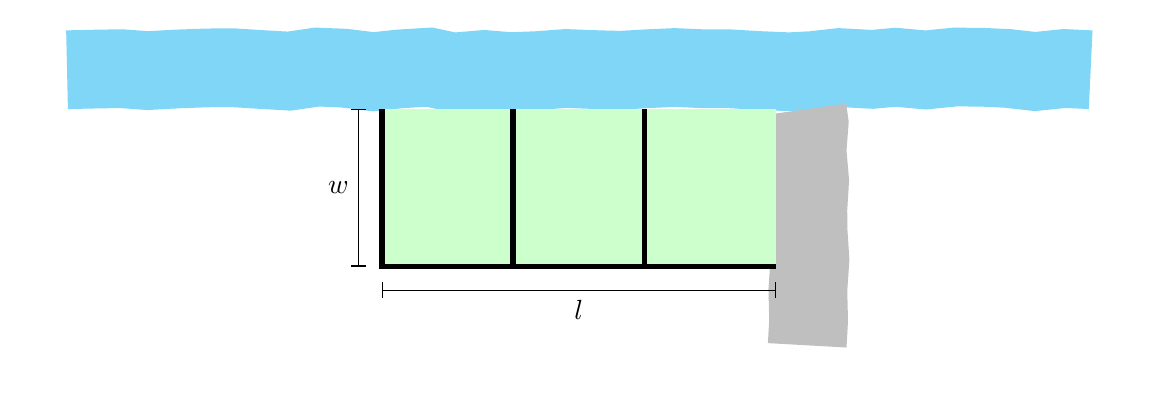
\begin{tikzpicture}[pencildraw/.style={decorate, decoration={random steps,segment length=10pt,amplitude=1pt}}]
		\pgfmathsetmacro\RiverWidth{1}
		\pgfmathsetmacro\RiverExtend{4}
		\pgfmathsetmacro\EnclosureLength{5}
		\pgfmathsetmacro\EnclosureWidth{2}
		\pgfmathsetmacro\InteriorFences{2}
		\pgfmathparse{\EnclosureLength/(\InteriorFences+1)}
		\pgfmathsetmacro\SubdivisionDistance{\pgfmathresult}
		% Set Coordinates
		\coordinate (R1) at (-\RiverExtend,\RiverWidth/2);
		\coordinate (R2) at (\EnclosureLength+\RiverExtend,\RiverWidth/2);
		\coordinate (EU1) at (0,0);
		\coordinate (EU2) at (\EnclosureLength,0);
		\coordinate (EL1) at ($ (EU1) + (0,-\EnclosureWidth) $);
		\coordinate (EL2) at ($ (EU2) + (0,-\EnclosureWidth) $);
                \coordinate (WS) at ($ (EU2) + (0.4,0) $);
                \coordinate (WE) at ($(EL2) + (0.4,- .5 * \EnclosureWidth) $);
		% Draw River
		\draw[cyan!50, line width=\RiverWidth cm, pencildraw] (R1) -- (R2);
		% Draw wall
		\draw[gray!50, line width=\RiverWidth cm, pencildraw] (WE) -- (WS);
		% Draw Rectangle
		\fill[green!20] (EU1) rectangle (EL2);
		% Draw Edges
		\draw[line width=2pt] (EU1) -- (EL1) -- (EL2);
		% Draw Subdivisions
		\ifthenelse{\InteriorFences>0}{
		\foreach \x in {1,...,\InteriorFences}{
			\draw[line width=2pt] ($ (EU1) + (\x*\SubdivisionDistance,0) $) -- ($ (EL1) + (\x*\SubdivisionDistance,0) $);
		}}{}
		% Label Enclosure
		\draw[|-|] ($ (EU1) + (-.3,0) $) -- +(0,-\EnclosureWidth) node[midway, left] {$w$};
		\draw[|-|] ($ (EL1) + (0,-.3) $) -- +(\EnclosureLength,0) node[midway, below] {$l$};
		\end{tikzpicture}
	\end{center}
\begin{enumerate}
\item Express total area enclosed as a function of $w$.
  \vspace{2in}
\item Roughly sketch the graph of this function, labeling your axes. What dimensions will maximize the area enclosed by this newly built pen? Why must this be a maximum?
  \\ \\
  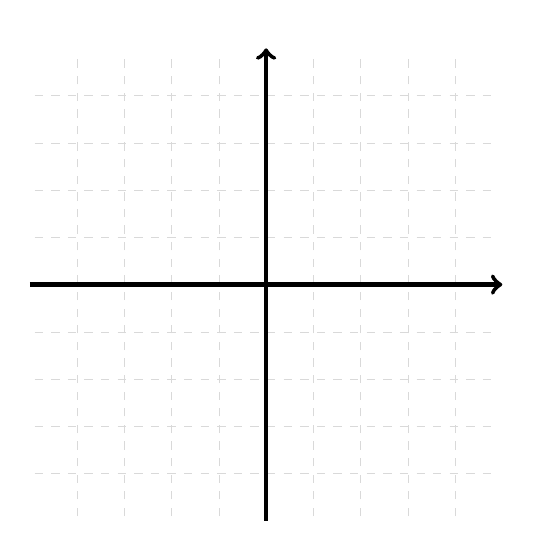
\begin{tikzpicture}[scale=0.6]
\draw[help lines, color=gray!30, dashed] (-4.9,-4.9) grid (4.9,4.9);
\draw[->,ultra thick] (-5,0)--(5,0) node[right]{};
\draw[->,ultra thick] (0,-5)--(0,5) node[above]{};

\end{tikzpicture}
\end{enumerate}


\end{document}
